%%%%% Techinical Preliminaries %%%%%

In this section I will give an overview of different 
mathematical and computational concepts
that we will use throughout the rest of this document. 
First, since we consider preference relations that are modeled
as binary relations,
we recall binary relations, properties of binary relations
and different preference relations satisfying some properties.
Second, we review combinatorial domains because we focus on
problems concerning preferences over combinatorial domains.
Finally, in order to quantify how hard these problems are in
a computational sense, we discuss concepts in computational
complexity theory that are related to our research.

\section{Relations \label{sec:relations}}


\begin{definition}
	Let $A$ and $B$ be two sets of elements.  A \textit{binary relation} $R$ between $A$ and $B$
	is a subset of the Cartesian product of $A$ and $B$, that is,
	\begin{center}
		$R \subseteq A \times B$.
	\end{center}
\end{definition}


Now let us review some of the important properties of binary relations.
\begin{definition}
	Let $R$ be a binary relation over a set $O$ of objects ($R \subseteq O \times O$),
	we define the following properties of $R$:
	\begin{enumerate} \itemsep -4pt
		\item reflexive: $\forall o \in O, oRo$.
		\item irreflexive: $\forall o \in O, \neg oRo$.
		\item total: $\forall o,o' \in O, oRo'$ or $o'Ro$.
		\item transitive: $\forall o,o',o'' \in O$, if $oRo'$ and $o'Ro''$, $oRo''$.
%		\item symmetric: $\forall o,o' \in O$, if $oRo'$, $o'Ro$.
		\item antisymmetric: $\forall o,o' \in O$, if $oRo'$ and $o \not = o'$, $\neg o'Ro$.
%		\item asymmetric: $\forall o,o' \in O$, if $oRo'$, $\neg o'Ro$.
	\end{enumerate}
\end{definition}

For instance, assuming $\bbN=\{1,2,\ldots\}$ is the set of positive integers,
the at-most relation $\leq$ over $\bbN$ is reflexive,
complete, transitive and antisymmetric, while the less-than relation
$<$ over $\bbN$ is irreflexive, transitive and antisymmetric.

\begin{definition}
\label{def:orders}
	A binary relation over $O$ is a \textit{partial preorder} if it is reflexive and transitive,
	a \textit{total preorder} if it is a partial preorder and total,
	a \textit{partial order} if it is a partial preorder and antisymmetric,
	or a \textit{total order} if it is a partial order and total.
\end{definition}

Preference relations can be modeled as binary relations as defined in \defref{orders}.
Given two objects $o$ and $o'$,
we sometimes need to specify that $o'$ is at least as good as $o$ or
$o'$ is strictly preferred over $o$.
In some situations we need to speak about the fact that $o'$ is
as good as $o'$, whereas in some other situations, due to some reasons
(e.g., lack of informations about the two objects at hand), we just
cannot determine which object is preferred over the other.  Formally,
we have the following definitions.
\begin{definition}
	Let $O$ be a set of objects, $o$ and $o'$ two objects in $O$.
	Let $\succeq$ be a preference relation that is a partial preorder \footnote{
		We only show the most general case where a preference relation is
		a partial preorder.  Other cases will be defined accordingly.
	}
	over $O$.
	We say that $o'$ is weakly preferred to $o$ if $o' \succeq o$.
	Object $o'$ is strictly preferred to $o$, $o' \succ o$, if $o' \succeq o$ and $o \not \succeq o'$.
	Object $o'$ is indifferent from $o$, $o' \approx o$, if $o' \succeq o$ and $o \succeq o'$.
	Object $o'$ is incomparable with $o$, $o' \sim o$, if $o' \not \succeq o$ and $o \not \succeq o'$.
\end{definition}

\nop{\tc{Examples of these orders.}}
Let us consider some examples of preference relations in \figref{relations}.
We assume that a directed edge between two objects is from the less preferred object to
the more preferred one.
We also assume that relations obtained by transitivity are omitted.
It is clear that the relation in \figref{relations}(a) is a partial 
order, and \figref{relations}(b) a total order.


\begin{figure}[ht]
   \small
  \centering
		\begin{subfigure}[b]{0.45\textwidth}
	  	\centering
		  \begin{tikzpicture}[->,>=stealth',node distance=1.5cm,main node/.style={circle,draw,font=\small}]
		    \node[main node,inner sep=0pt] (1)                    {$o_1,\!o_5$};
				\node[main node,inner sep=0pt] (2) [below left of=1]  {$o_2,\!o_6$};
		  	\node[main node,inner sep=0pt] (3) [below right of=1] {$o_3,\!o_7$};
		  	\node[main node,inner sep=0pt] (4) [below right of=2] {$o_4,\!o_8$};
		
		    \path[every node/.style={font=\sffamily\small}]
		      (4) edge (2)
		      (4) edge (3)
		      (2) edge (1)
		      (3) edge (1)
		      (4) edge (1)
					(1) edge [loop above] (1)
					(2) edge [loop left] (2)
					(3) edge [loop right] (3)
					(4) edge [loop below] (4);
		  \end{tikzpicture}
      \caption{partial preorder}
    \end{subfigure}
    \begin{subfigure}[b]{0.45\textwidth}
	  	\centering
		  \begin{tikzpicture}[->,>=stealth',node distance=1.1cm,main node/.style={circle,draw,font=\small}]
		    \node[main node,inner sep=0pt] (1)              {$o_1,\!o_5$};
				\node[main node,inner sep=0pt] (2) [below of=1] {$o_2,\!o_6$};
		  	\node[main node,inner sep=0pt] (3) [below of=2] {$o_3,\!o_7$};
		  	\node[main node,inner sep=0pt] (4) [below of=3] {$o_4,\!o_8$};
		
		    \path[every node/.style={font=\sffamily\small}]
		      (4) edge (3)
		      (4) edge [bend left] (2)
		      (4) edge [bend left] (1)
		      (3) edge (2)
		      (3) edge [bend left] (1)
		      (2) edge (1)
					(1) edge [loop right] (1)
					(2) edge [loop right] (2)
					(3) edge [loop right] (3)
					(4) edge [loop right] (4);
		  \end{tikzpicture}
      \caption{total preorder}
    \end{subfigure} \\
    \begin{subfigure}[b]{0.45\textwidth}
	  	\centering
		  \begin{tikzpicture}[->,>=stealth',node distance=1.5cm,main node/.style={circle,draw,font=\small}]
		    \node[main node] (1) {$o_1$};
				\node[main node] (2) [below left of=1] {$o_2$};
		  	\node[main node] (3) [below right of=1] {$o_3$};
		  	\node[main node] (4) [below right of=2] {$o_4$};
		
		    \path[every node/.style={font=\sffamily\small}]
		      (4) edge (2)
		      (4) edge (3)
		      (2) edge (1)
		      (3) edge (1)
		      (4) edge (1)
					(1) edge [loop above] (1)
					(2) edge [loop left] (2)
					(3) edge [loop right] (3)
					(4) edge [loop below] (4);
		  \end{tikzpicture}
      \caption{partial order}
    \end{subfigure}
    \begin{subfigure}[b]{0.45\textwidth}
	  	\centering
		  \begin{tikzpicture}[->,>=stealth',node distance=1cm,main node/.style={circle,draw,font=\small}]
		    \node[main node] (1) {$o_1$};
				\node[main node] (2) [below of=1] {$o_2$};
		  	\node[main node] (3) [below of=2] {$o_3$};
		  	\node[main node] (4) [below of=3] {$o_4$};
		
		    \path[every node/.style={font=\sffamily\small}]
		      (4) edge (3)
		      (4) edge [bend left] (2)
		      (4) edge [bend left] (1)
		      (3) edge (2)
		      (3) edge [bend left] (1)
		      (2) edge (1)
					(1) edge [loop right] (1)
					(2) edge [loop right] (2)
					(3) edge [loop right] (3)
					(4) edge [loop right] (4);
		  \end{tikzpicture}
      \caption{total order}
    \end{subfigure}
  \caption{Binary relations}
  \label{fig:relations}
\end{figure}


\begin{definition}
	Let $R$ and $R'$ be two binary relations,
	$R'$ \textit{extends} $R$ if $R \subseteq R'$.
\end{definition}

As an example of relation extensions, we consider the partial order $\succeq$ 
in \figref{relations}(a).
Since $o_2 \sim o_3$, we have in total two extensions:
\begin{center}
	$o_1 \succeq o_2 \succeq o_3 \succeq o_4$,\\
	$o_1 \succeq o_3 \succeq o_2 \succeq o_4$.
\end{center}

\begin{definition}
	Let $\succeq$ be a preference relation over $O$,
	$o \in O$ is \textit{maximal} if there exists $o' \in O$
	such that $o' \succeq o$.
\end{definition}
For instance, object $o_1$ is maximal in the total order
shown in \figref{relations}(b).



\section{Combinatorial Domains \label{sec:comb_domains}}
%One thing that makes decision problems difficult is the fact that outcomes of preferences 
%are usually not represented directly as a given set of objects.
%We focus on preferences among outcomes from combinatorial domains \cite{bbdh03}.
We define the combinatorial domain as follows.

\begin{definition}
	Let $\bV$ be a set of variables (or features, attributes) $\{X_1,\ldots,X_p\}$,
	$\bD$ a set of finite domains $\{\Dom(X_1),\ldots,\Dom(X_p)\}$ for each
	variable $X_i$.
	A \textit{combinatorial domain} is a triple $\langle \bV, \bD, \bT \rangle$,
	where $\bT$ is a set of tuples that are combinations of values from
	domains in $\bD$ of variables in $\bV$:
	\begin{center}
		$\bT = \prod_{X_i \in \bV} \Dom(X_i)$.
	\end{center}
\end{definition}

An example of combinatorial domain is the space of \textit{subsets} of $\bV$.
In this case, $\bD$ is a set of binary domains, and a tuple
$t \in \bT$ is a combination of 0's and 1's.
Note that $0_i \in t$ means that $X_i$ is not in the corresponding subset,
and that $1_i \in t$ means that $X_i$ is.
It is not hard to see that
the set $\bT$ of tuples is exactly the space $\bS$ of subsets of $\bV$.

Clearly, the size of $\bT$ is exponential in $p$, the number of variables.
Note that, even though sets $\bV$ of binary variables are of main interest,
the exponential growth of $|\bV|$ makes it impossible for agents
to directly assess their preferences.
Also notice that, in many practical cases, hard constraints (e.g., propositional
formulas) are identified to eliminate the infeasible outcomes.



\section{Computational Complexity Theory \label{sec:comp_theory}}
\nop{\tc{
Here I talk about complexity classes of interest, including
the classes P, NP, coNP, NP-complete, coNP-complete, NP-Hard, \#P, polynomial
hierarchy.
}}

Computer scientists looking for algorithms to solve computational problems
seek ways to classify problems according to their computational hardness
in terms of time (the number of instructions needed to solve the problem) 
or space (the size of memory needed to solve the problem).
In this section, I define classes of computational
complexity used for such classification.
We assume formiliarity with the concept of the \textit{Turing machine} (TM).
Details of it and other definitions discussed below can be found in complexity
books by Garey and Johnson \cite{gar-joh:b:int}; Lewis and Papadimitriou
\cite{Lewis:Comput}; and Arora and Barak \cite{Arora:Comput}.



\subsection{Decision Problems}
Let $\Sigma$ be a finite set of elements, a string over alphabet $\Sigma$
is an ordered tuple of finite elements from $\Sigma$. In complexity theory,
$\Sigma$ is typically binary, that is, $\Sigma=\{0,1\}$.
We denote by $\Sigma^*$ the set of all strings of elements in $\Sigma$.

\begin{definition}
	Let $f$ be a TM.
	A \textit{decision problem} (or a \textit{language}) is a set 
	$L_f$ of strings ($L \subseteq \Sigma^*$) such that $f$ accepts
	any string in $L_f$.
\end{definition}
For instance, the SAT problem is the set of all finite propositional
formulas that have a satisfying truth assignment (assuming some natural
representation of propositional formulas as strings over a finite alphabet).



\subsection{$\bP$, $\bNP$ and $\bCoNP$}
What differentiates the two classes $\bP$ and $\bNP$ is whether the decision problem
can be solved by a deterministic or a nondeterministic TM. \cite{Arora:Comput}
%A \textit{deterministic} TM is a TM that, for any given input, always proceeds the
%computation in exactly one way.
%A \textit{nondeterministic} TM, however, consists of two phases:
%(1). guess about the solution which is in a nondeterministic way,
%and (2). verifies or rejects the guess as a valid solution to the problem.

%In general, we classify complexity classes with regard to computational resources
%needed in the process of solving the problem, i.e., time and space.
%We focus on complexity classes with respect to ``time," although
%we will discuss about the class of PSPACE with respect to ``space" in a
%later section.
Let $\bDTIME(x)$ ($\bNTIME(x)$) be a set of decision problems 
for which there exists a deterministic (nondeterministic, respectively) TM
that solves any instance of the problems in time $c\cdot x$ for some
constant $c>0$.
We now define the two classes as follows.

\begin{definition}
	The class $\bP$ ($\bNP$) contains the decision problems that can be solved using a 
	deterministic (nondeterministic, respectively) TM 
	in time polynomial in the size of the input.  Formally, we have
	\begin{center}
		$\bP = \bigcup_{d \in \bbN} \bDTIME(n^d)$,\\
		$\bNP = \bigcup_{d \in \bbN} \bNTIME(n^d)$,
	\end{center}
	where $n$ is the size of the input.
\end{definition}

Researchers in the field of complexity theory have studied
the relation between these two classes.
%Intuitively, class $\bP$ speaks about the efficiency of a TM
%in finding a correct solution, whereas class $\bNP$, in
%verifying the correctness of a proposed solution.
Clearly, the relation $\bP \subseteq \bNP$ holds. Whether
$\bNP \subseteq \bP$ holds or not remains an open question.
However, it is mostly believed that $\bP \not = \bNP$ \cite{gasarch2002p}. 


One of the many complexity classes related to $\bP$ and $\bNP$ \cite{gasarch2002p}
is the class $\bCoNP$, which contains problems that are complement of 
the problems in $\bNP$.
Let $L \subseteq \{0,1\}^*$ be a decision problem, we denote by $\overline{L}$ the
complement of $L$, that is, $\overline{L} = \{0,1\}^*-L$.
We have the following definition of the class $\bCoNP$.

\begin{definition}
	$\bCoNP = \{L : \overline{L} \in \bNP\}$.
\end{definition}

To characterize the most difficult problems in class $C$ ($\bNP$, $\bCoNP$, etc), 
it is helpful to introduce
the definition of polynomial-time reducibility \cite{gasarch2002p} and the 
idea of $C$-hardness.

\begin{definition}
	A decision problem $L \subseteq \{0,1\}^*$  is \textit{polynomial-time reducible} to
	a decision problem $L' \subseteq \{0,1\}^*$, $L \leq_p L'$, if there is a
	polynomial-time computable function $g : \{0,1\}^* \rightarrow \{0,1\}^*$
	such that for every instance $x \in L$ $\itiff$ $f(x) \in L'$.
	We say that $L'$ is $C$-\textit{hard} if $L \leq_p L'$ for every $L$ in class $C$.
\end{definition}

%This hardness expresses the idea that problem $L'$ is at least at hard as
%every problem in class $C$ and consequently $L'$ might not even belong to $C$.

\begin{definition}
	Let $C$ be a complexity class ($\bNP$, $\bCoNP$, etc).
	A decision problem $L'$ is $C$-\textit{complete} if $L'$ is in class $C$ and $L'$ is $C$-hard.
\end{definition}
It is clear that, in order to prove $C$-completeness, one need to first show
that $L' \in C$ (membership of class $C$), and then prove $C$-hardness.



\subsection{TM with Oracles and Polynomial Hierarchy}
%Some decision problems are harder than problems in classes $\bP$, $\bNP$ and $\bCoNP$
%in the sense that solving these problems involves oracle machines for complete
%problems in those three classes.
%For this reason, the classes of the polynomial hierarchy are defined, inductively.
%\noindent{\textbf{TM with Oracles.}}
A \textit{TM with an oracle} for a decision problem $L$ is a TM that makes calls to an algorithm that
decides $L$.

\begin{definition}
	Define the base case:
	\begin{center}
		$\deltap{0} = \sigmap{0} = \pip{0} = \bP$,
	\end{center}
	Then for $i \geq 0$, we denote by $\deltap{i+1}$ ($\sigmap{i+1}$) 
	the set of decision problems solvable
	by a deterministic (nondeterministic, respectively) TM 
	in polynomial time with an oracle for some $\sigmap{i}$-complete problem.
	We denote by $\pip{i+1}$ the set of decision problems that are complement
	of problems in $\sigmap{i+1}$.
%	\begin{center}
%		$\deltap{i+1} = \bP^{\sigmap{i}}$, \\
%		$\sigmap{i+1} = \bNP^{\sigmap{i}}$, \\
%		$\pip{i+1} = \bCoNP^{\sigmap{i}}$.
%	\end{center}
\end{definition}
For example, $\sigmap{2}$ is the class of decision problems solvable by a nondeterministic
TM in polynomial time with an oracle for some $\bNP$-complete problem.
We denote by $\bPH$ the collection of all classes in the polynomial hierarchy.

The relation between any classes on the hierarchy is of interest.
One may notice that the classes $\sigmap{i}$ and $\pip{i}$ are
complement, that is $\sigmap{i} = \textbf{co}\pip{i}$.
Moreover, we have the relations of these classes as shown in \figref{ph_diagram}.

\begin{figure}[h!]
  \centering
  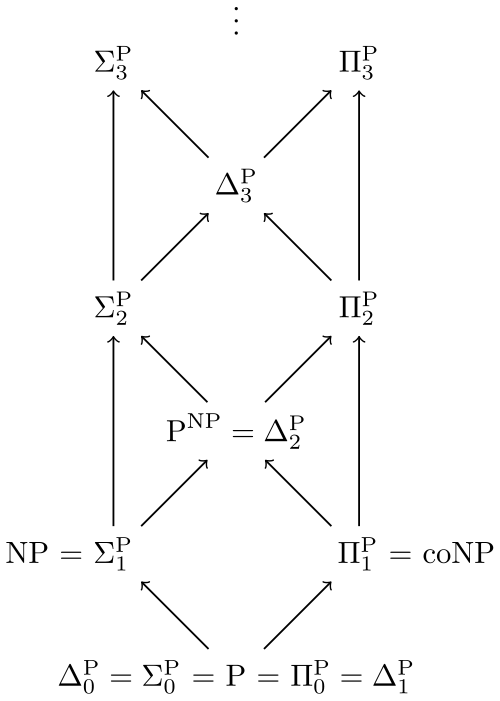
\includegraphics[width=0.3\textwidth]{img/ph_diagram.png}
  \caption{Polynomial hierarchy diagram \label{fig:ph_diagram}}
\end{figure}


\subsection{$\bPSPACE$}
In this work, we consider yet another complexity class we will 
use later is $\bPSPACE$ that
concerns the complexity of space.

\begin{definition}
	The class $\bPSPACE$ is the class of decision problems solvable by a TM
	in space polynomial in the size of the input.
\end{definition}
It is not hard to see the following relation hold.
\begin{center}
	$\bPH \subseteq \bPSPACE$.
\end{center}

We illustrate the relationship among the complexity classes in
\figref{comp_diagram}. Many classes are omitted in our diagram
that are not in our focus.

\begin{figure}[h!]
  \centering
  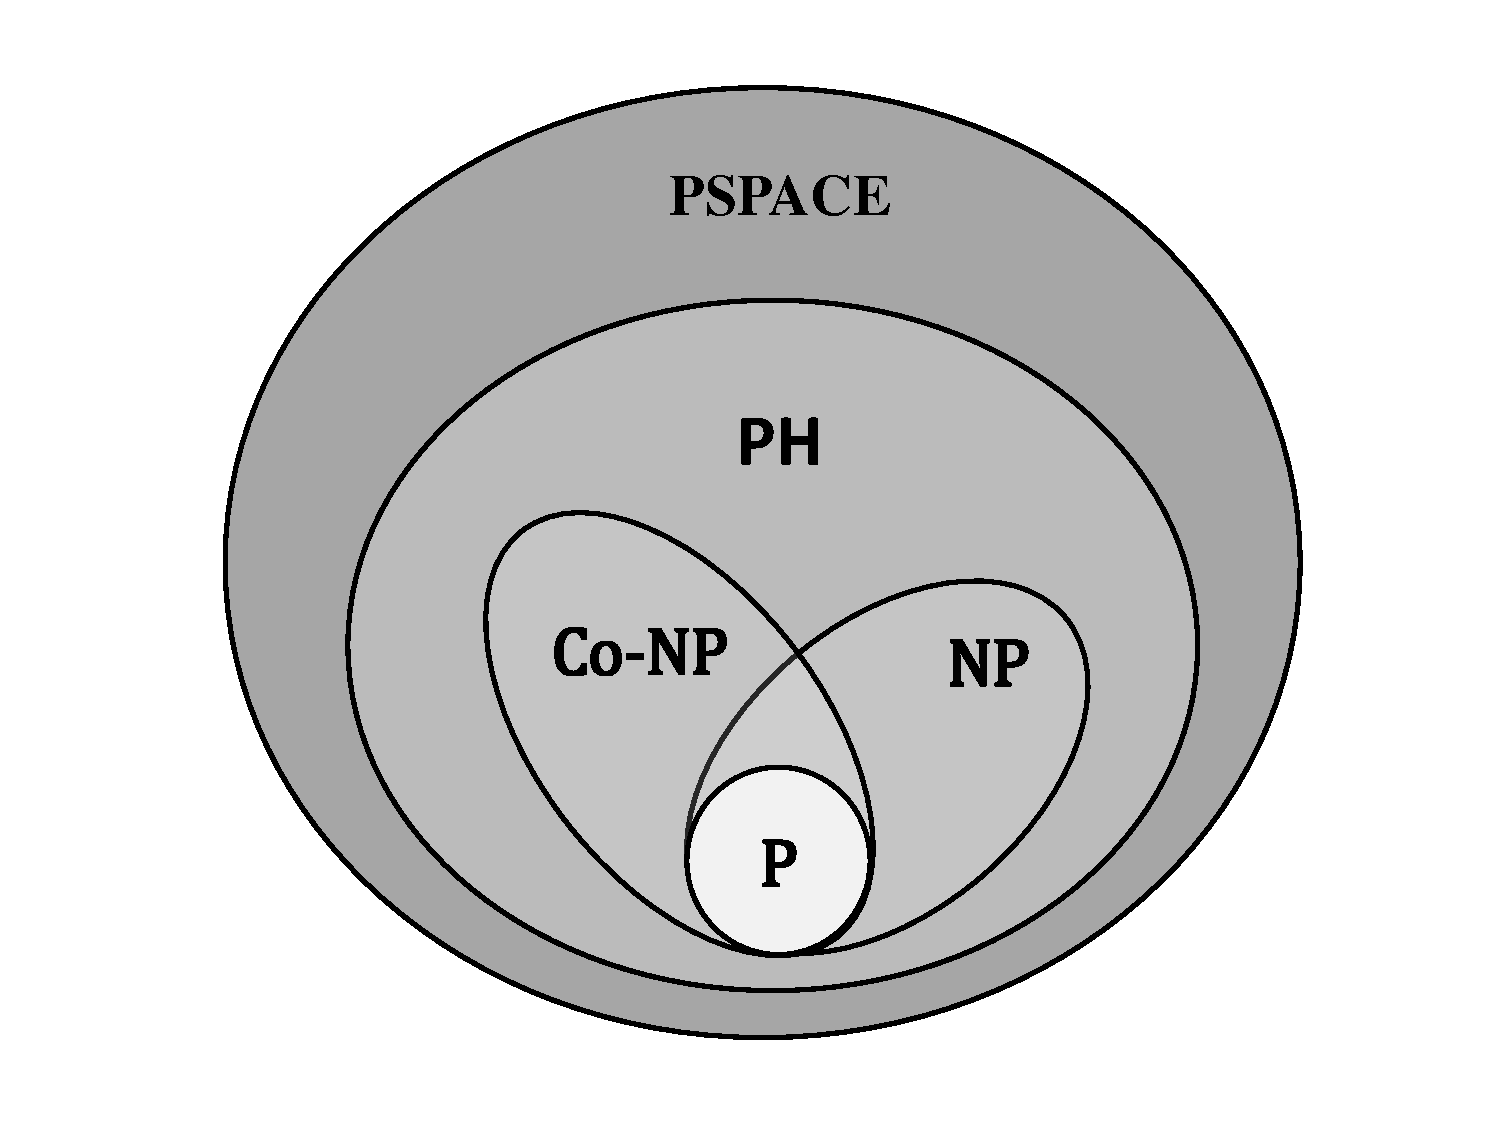
\includegraphics[width=0.7\textwidth]{img/comp_diagram.pdf}
  \caption{Computational complexity diagram \label{fig:comp_diagram}}
\end{figure}
